% Chapter 1
\stepcounter{cap}
%\chapter{cap1}
\label{cap6}

\mychapter{6}{Capitolul \arabic{cap} \\ CONCLUZII}
%\chapter{\arabic{cap}.Introducere} % Main chapter title

\label{Chapter6} % For referencing the chapter elsewhere, use \ref{Chapter1} 

\thispagestyle{fancy}

%-----------------------------------------------------------------

\section{Concluzii generale} 
Scopul acestei lucrări a fost acela de a dezvolta un modul de navigare pentru estimarea rutelor posibile ale unui autovehicul. Fiind într-o lume în continuă mișcare și în care orice autovehicul modern dispune de o aplicație de navigare, s-a dorit oferirea utilizatorului de servicii care să-i ușureze acestuia munca și să transforme experiența utilizării unei astfel de produs într-o plăcere.
\vspace{6pt}
\\În cadrul lucrării au fost prezentate deciziile cu cea mai mare influență asupra proiectului, definirea arhitecturii modului, logica din spatele algoritmilor dar bineînțeles și eventualele erori ce pot să apară și soluții aferente prevenirii lor.
\vspace{6pt}
\\Pentru realizarea proiectului s-a folosit limbajul de programare C++. S-a făcut această alegere deoarece este unul dintre limbajele cel mai bine stăpânite, dar și datorită faptului se dispunea deja de o aplicație de navigare scrisă în C++, lucrul ce a făcut ca dezvoltarea, integrarea și testarea modulului să fie mult mai facilă.
\vspace{6pt}
\\Primul pas a fost bineînțeles stabilirea clară a funcționalităților ce se doresc a fi obținute de la modulul în cauză. Odată deciși asupra acestori factori s-a creat diagrama de design software pe baza căreia, mai târziu, s-a început definirea unităților software și scrierea codului în sine. Până la scrierea codului însă au fost necesare și luarea anumitor decizii, precum alegerea tipului de bază de date. În urma alegerii făcute a fost realizată și o scurtă documentare asupra modului cum poate fi folosit \acrshort{api}-ul acesteia pentru crearea legăturii și comunicarea efectivă dintre partea de cod și baza de date în sine.
\vspace{6pt}
\\Din punct de vedere al funcționalității, modulul a fost împărțit în două, prima parte fiind învățarea rutelor iar a doua predicția acestora.
\vspace{6pt}
\\Prin învățarea se înțelege stocarea datelor colectate pe parcursul rutelor frecventate de utilizator. Pentru ca baza de date rezultată să fie însă atât compactă cât și încărcată cât mai rapid, s-a optat pentru un mod de învățare inteligentă, prin aplicarea unor algoritmi de constrângere ce au ca scop filtrarea acestor date în funcții de anumite criterii.
\vspace{6pt}
\\Pe partea de predicție a rutelor pot exista diverse abordări și rezultate dorite din partea celui ce folosește modulul în cadrul aplicație sale, așa că pe lângă valorile standard s-a oferit și posibilitatea de configurare a criteriilor ce stau la baza mecanismului de predicție.
\vspace{6pt}
\\Ca și concluzie finală putem spune că s-a dezvoltat un modul ambalat sub forma unei biblioteci cu legare dinamică (\acrshort{dll}), configurabil și utilizabil în cadrul oricărei aplicații de navigare, ce colectează date despre rute și oferă la rândul său predicții pe baza acestora.

\section{Posibilități de dezvoltare ulterioară} 
În urma realizării acestui proiect, a studierii necesităților și așteptărilor utilizatorului comun de la un sistem de navigație, dar și a analizei soluțiilor deja existente se pot indica mai multe direcții de dezvoltare.
\vspace{6pt}
\\O posibilă direcție de dezvoltare ar putea fi folosirea acestui modul împreună cu un altul de furnizare al datelor de trafic.
\vspace{6pt}
\\Presupunem faptul că utlizatorul este pe ruta folosită de acesta în mod uzual însă la un alt moment de timp față de obicei, moment în care traficul este mult mai intens pe tronsonul respectiv de drum.
Folosind datele furnizate de cele două module, utilizatorului i se va putea oferi posibilitatea de a alege o rută alternativă, mult mai rapidă.

\begin{figure}[h!]
  \centering
   \centering{%
   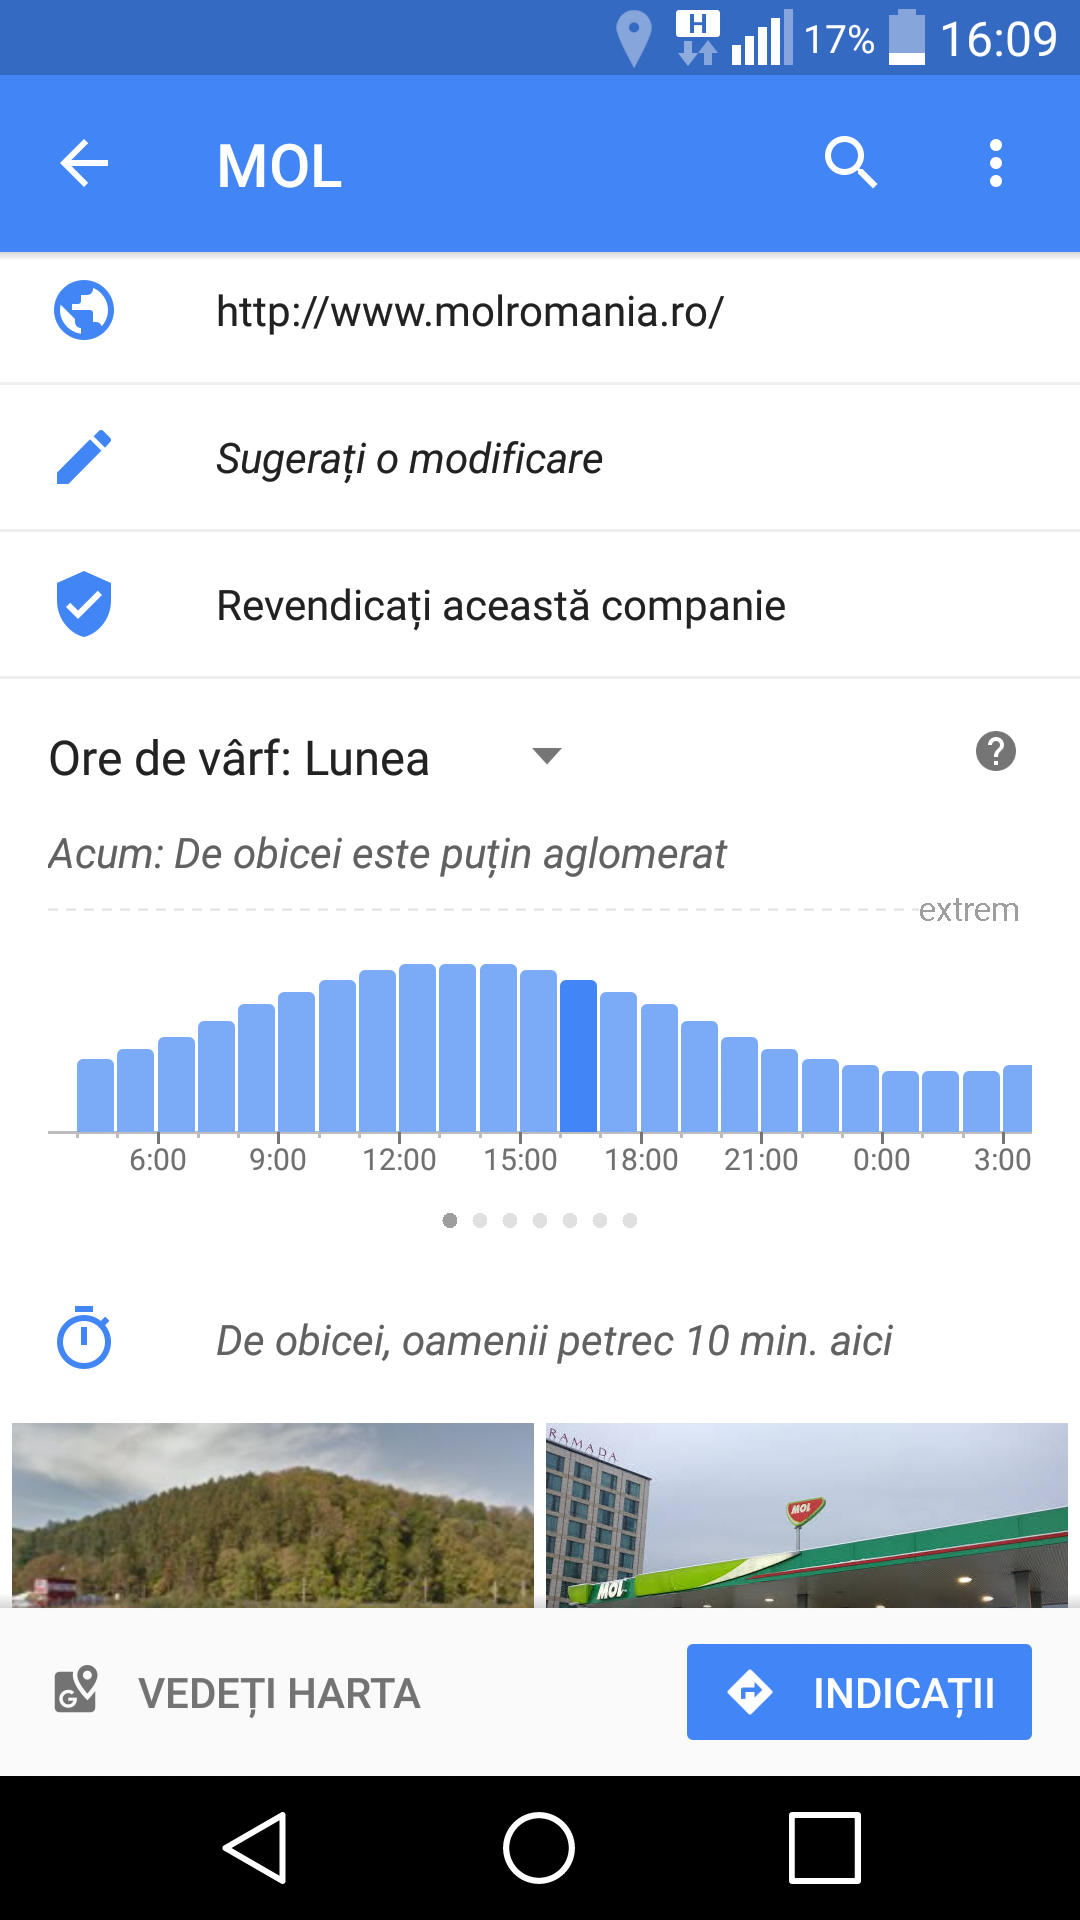
\includegraphics[width=0.4\textwidth]{Figures/mol.png}}
  \caption{Captură de ecran din aplicația Google Maps}
  \end{figure}	
  
Același principiu s-ar putea aplica și pentru alte evenimente întâlnite în trafic, precum accidente, lucrări în desfășurare, și așa mai departe.
\vspace{6pt}
\\O altă direcție de dezvoltare ar fi crearea unei extensii pentru modul, cu scopul de a se sincroniza cu dispozitivul utilizatorului (e.g. telefon înteligent) și de a prelua evenimentele planificate în calendarul acestuia. Fiind astfel extinsă funcționalitatea modulului, utilizatorului i se vor putea oferi predicții și pe baza planificărilor făcute de acesta anterior.

\begin{figure}[h!]
  \centering
   \centering{%
   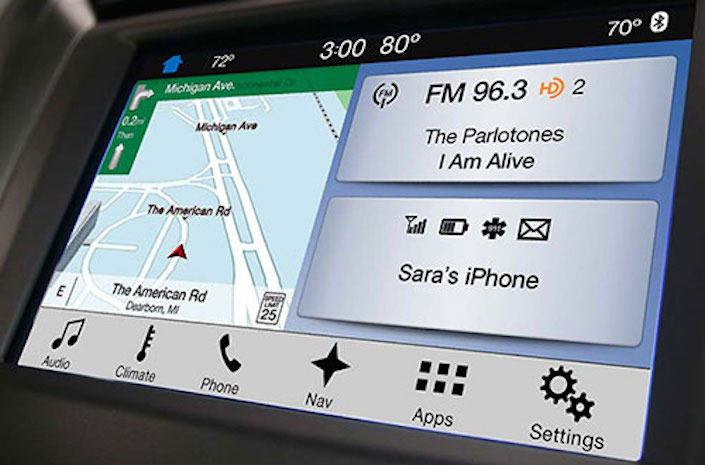
\includegraphics[width=0.6\textwidth]{Figures/ford_sinc.jpg}}
  \caption{Sincronizarea între un sistem de navigare de pe Ford XL 2014 și un telefon inteligent}
  \end{figure}	

Bineînțeles, cum industria automobilistică este una în continuă evoluție vor apărea întotdeauna noi oportunități de dezvoltare a aplicațiilor de navigare și implicit a modulului în sine.